%%% Hlavní soubor. Zde se definují základní parametry a odkazuje se na ostatní části. %%%

%% Verze pro jednostranný tisk:
% Okraje: levý 40mm, pravý 25mm, horní a dolní 25mm
% (ale pozor, LaTeX si sám přidává 1in)
\documentclass[12pt,a4paper]{report}
\setlength\textwidth{145mm}
\setlength\textheight{247mm}
\setlength\oddsidemargin{15mm}
\setlength\evensidemargin{15mm}
\setlength\topmargin{0mm}
\setlength\headsep{0mm}
\setlength\headheight{0mm}
% \openright zařídí, aby následující text začínal na pravé straně knihy
\let\openright=\clearpage

%% Pokud tiskneme oboustranně:
% \documentclass[12pt,a4paper,twoside,openright]{report}
% \setlength\textwidth{145mm}
% \setlength\textheight{247mm}
% \setlength\oddsidemargin{14.2mm}
% \setlength\evensidemargin{0mm}
% \setlength\topmargin{0mm}
% \setlength\headsep{0mm}
% \setlength\headheight{0mm}
% \let\openright=\cleardoublepage

%% Vytváříme PDF/A-2u
\usepackage[a-2u]{pdfx}

%% Přepneme na českou sazbu a fonty Latin Modern
%\usepackage[czech]{babel}
\usepackage{lmodern}
\usepackage[T1]{fontenc}
\usepackage{textcomp}

%% Použité kódování znaků: obvykle latin2, cp1250 nebo utf8:
\usepackage[utf8]{inputenc}

%%% Další užitečné balíčky (jsou součástí běžných distribucí LaTeXu)
\usepackage{amsmath}        % rozšíření pro sazbu matematiky
\usepackage{amsfonts}       % matematické fonty
\usepackage{amsthm}         % sazba vět, definic apod.
\usepackage{bbding}         % balíček s nejrůznějšími symboly
			    % (čtverečky, hvězdičky, tužtičky, nůžtičky, ...)
\usepackage{bm}             % tučné symboly (příkaz \bm)
\usepackage{graphicx}       % vkládání obrázků
\usepackage{fancyvrb}       % vylepšené prostředí pro strojové písmo
\usepackage{indentfirst}    % zavede odsazení 1. odstavce kapitoly
\usepackage{natbib}         % zajištuje možnost odkazovat na literaturu
			    % stylem AUTOR (ROK), resp. AUTOR [ČÍSLO]
\usepackage[nottoc]{tocbibind} % zajistí přidání seznamu literatury,
                            % obrázků a tabulek do obsahu
\usepackage{icomma}         % inteligetní čárka v matematickém módu
\usepackage{dcolumn}        % lepší zarovnání sloupců v tabulkách
\usepackage{booktabs}       % lepší vodorovné linky v tabulkách
\usepackage{paralist}       % lepší enumerate a itemize
\usepackage{xcolor}         % barevná sazba

\usepackage{rotating}
%\usepackage{fontspec}
\usepackage{tipa}
\usepackage{enumitem}
\usepackage{makecell}
\usepackage{alltt}
\usepackage{refcount}
\usepackage{tabularx}
\usepackage{caption}


%%% Údaje o práci

% Název práce v jazyce práce (přesně podle zadání)
\def\NazevPrace{Iterativní zdokonalování přepisu zvukových nahrávek s~využitím zpětné vazby posluchačů}

% Název práce v angličtině
\def\NazevPraceEN{Iterative Improving of Transcribed Speech Recordings Exploiting Listener's Feedback}

% Jméno autora
\def\AutorPrace{Mgr. Jan Oldřich Krůza}

% Rok odevzdání
\def\RokOdevzdani{2020}

% Název katedry nebo ústavu, kde byla práce oficiálně zadána
% (dle Organizační struktury MFF UK, případně plný název pracoviště mimo MFF)
\def\Katedra{Ústav formální a aplikované lingvistiky}
\def\KatedraEN{Institute of Formal and Applied Linguistics}

% Jedná se o katedru (department) nebo o ústav (institute)?
\def\TypPracoviste{Ústav}
\def\TypPracovisteEN{Institute}

% Vedoucí práce: Jméno a příjmení s~tituly
\def\Vedouci{Doc. RNDr. Vladislav Kuboň, Ph.D.}

% Pracoviště vedoucího (opět dle Organizační struktury MFF)
\def\KatedraVedouciho{
  Ústav formální a aplikované lingvistiky\\
  Matematicko-fyzikální fakulta\\
  Univerzita Karlova\\
  Malostranské náměstí 25\\
  11800 Praha 1
}
\def\KatedraVedoucihoEN{Institute of Formal and Applied Linguistics}

% Studijní program a obor
\def\StudijniProgram{informatika}
\def\StudijniObor{matematická lingvistika}

%% Balíček hyperref, kterým jdou vyrábět klikací odkazy v PDF,
%% ale hlavně ho používáme k uložení metadat do PDF (včetně obsahu).
%% Většinu nastavítek přednastaví balíček pdfx.
\hypersetup{unicode}
\hypersetup{breaklinks=true}

%% Definice různých užitečných maker (viz popis uvnitř souboru)
%%% Tento soubor obsahuje definice různých užitečných maker a prostředí %%%
%%% Další makra připisujte sem, ať nepřekáží v ostatních souborech.     %%%

%%% Drobné úpravy stylu

% Tato makra přesvědčují mírně ošklivým trikem LaTeX, aby hlavičky kapitol
% sázel příčetněji a nevynechával nad nimi spoustu místa. Směle ignorujte.
\makeatletter
\def\@makechapterhead#1{
  {\parindent \z@ \raggedright \normalfont
   \Huge\bfseries \thechapter. #1
   \par\nobreak
   \vskip 20\p@
}}
\def\@makeschapterhead#1{
  {\parindent \z@ \raggedright \normalfont
   \Huge\bfseries #1
   \par\nobreak
   \vskip 20\p@
}}
\makeatother

% Toto makro definuje kapitolu, která není očíslovaná, ale je uvedena v obsahu.
\def\chapwithtoc#1{
\chapter*{#1}
\addcontentsline{toc}{chapter}{#1}
}

% Trochu volnější nastavení dělení slov, než je default.
\lefthyphenmin=2
\righthyphenmin=2

% Zapne černé "slimáky" na koncích řádků, které přetekly, abychom si
% jich lépe všimli.
%\overfullrule=1mm

%%% Makra pro definice, věty, tvrzení, příklady, ... (vyžaduje baliček amsthm)

\theoremstyle{plain}
\newtheorem{veta}{Věta}
\newtheorem{lemma}[veta]{Lemma}
\newtheorem{tvrz}[veta]{Tvrzení}

\theoremstyle{plain}
\newtheorem{definice}{Definice}

\theoremstyle{remark}
\newtheorem*{dusl}{Důsledek}
\newtheorem*{pozn}{Poznámka}
\newtheorem*{prikl}{Příklad}

%%% Prostředí pro důkazy

\newenvironment{dukaz}{
  \par\medskip\noindent
  \textit{Důkaz}.
}{
\newline
\rightline{$\qedsymbol$}
}

%%% Prostředí pro sazbu kódu, případně vstupu/výstupu počítačových
%%% programů. (Vyžaduje balíček fancyvrb -- fancy verbatim.)

\DefineVerbatimEnvironment{code}{Verbatim}{fontsize=\small, frame=single}

%%% Prostor reálných, resp. přirozených čísel
\newcommand{\R}{\mathbb{R}}
\newcommand{\N}{\mathbb{N}}

%%% Užitečné operátory pro statistiku a pravděpodobnost
\DeclareMathOperator{\pr}{\textsf{P}}
\DeclareMathOperator{\E}{\textsf{E}\,}
\DeclareMathOperator{\var}{\textrm{var}}
\DeclareMathOperator{\sd}{\textrm{sd}}

%%% Příkaz pro transpozici vektoru/matice
\newcommand{\T}[1]{#1^\top}

%%% Vychytávky pro matematiku
\newcommand{\goto}{\rightarrow}
\newcommand{\gotop}{\stackrel{P}{\longrightarrow}}
\newcommand{\maon}[1]{o(n^{#1})}
\newcommand{\abs}[1]{\left|{#1}\right|}
\newcommand{\dint}{\int_0^\tau\!\!\int_0^\tau}
\newcommand{\isqr}[1]{\frac{1}{\sqrt{#1}}}

%%% Vychytávky pro tabulky
\newcommand{\pulrad}[1]{\raisebox{1.5ex}[0pt]{#1}}
\newcommand{\mc}[1]{\multicolumn{1}{c}{#1}}


%% Titulní strana a různé povinné informační strany
\begin{document}
%%% Titulní strana práce a další povinné informační strany

%%% Titulní strana práce

\pagestyle{empty}
\hypersetup{pageanchor=false}

\begin{center}

\centerline{\mbox{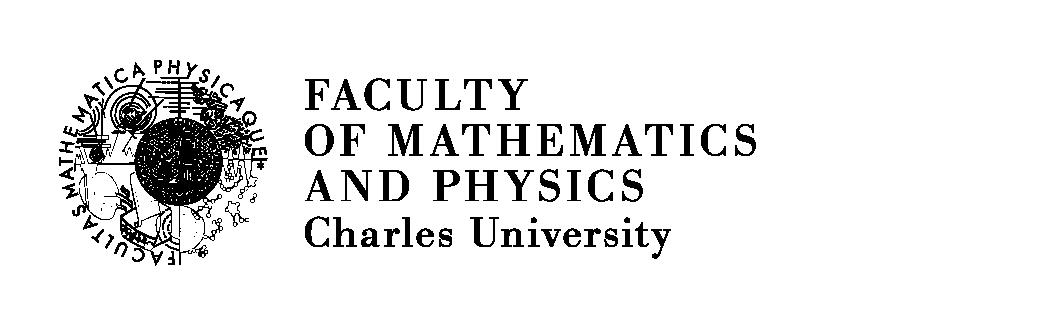
\includegraphics[width=166mm]{../img/logo-en.pdf}}}

\vspace{-8mm}
\vfill

{\bf\Large ABSTRACT OF DOCTORAL THESIS}

\vfill

{\LARGE\AutorPrace}

\vspace{15mm}

{\LARGE\bfseries\NazevPraceEN}

\vfill

\KatedraEN

\vfill

{
\centerline{\vbox{\halign{\hbox to 0.45\hsize{\hfil #}&\hskip 0.5em\parbox[t]{0.45\hsize}{\raggedright #}\cr
Supervisor:&\Vedouci \cr
\noalign{\vspace{2mm}}
Study programme:&Computer science \cr
\noalign{\vspace{2mm}}
Branch:& Computational linguistics\cr
}}}}

\vfill

% Zde doplňte rok
Praha \RokOdevzdani

\end{center}

\newpage

%%% Povinná informační strana disertační práce

\openright

\vbox to 0.5\vsize{
\setlength\parindent{0mm}
\setlength\parskip{5mm}

The results of this thesis were achieved in the pediod of a doctoral study at
the Faculty of Mathematics and Physics, Charles University in years
2011 -- 2020.

\vspace{2cm}

{
\centerline{\vbox{\halign{\hbox to 0.45\hsize{\hfil #}&\hskip 0.5em\parbox[t]{0.45\hsize}{\raggedright #}\cr
Student:&
\AutorPrace
\cr \noalign{\vspace{7mm}}
Supervisor:&
\Vedouci, \KatedraVedoucihoEN
\cr \noalign{\vspace{7mm}}
Department:&
\KatedraVedoucihoEN
\cr \noalign{\vspace{7mm}}
Opponents:&
Prof. Ing. Luděk Müller, Ph.D.\\
Fakulta aplikovaných věd ZČU, Katedra kybernetiky\\
Technická 8, 30614 Plzeň
\cr \noalign{\vspace{7mm}}
&Doc. Ing. Petr Pollák, CSc.\\
ČVUT FEL K13131,\\
Technická 2, 16627 Praha 6
\cr
}}}}

The thesis defense will take place on September 30th 2020 at 11:00 a.m. in front of a
committee for thesis defenses in the branch P4I3 Computational linguistics
at the Faculty of Mathematics and Physics, Charles University in
Prague, Malostranské náměstí 25, in the room S510.

The thesis can be viewed at the Study Department of Doctoral Studies of the Faculty of
Mathematics and Physics, Charles University in Prague, Ke Karlovu 3, Prague 2.

This abstract has been distributed on September 23rd 2020.

\vss}\nobreak\vbox to 0.49\vsize{
\setlength\parindent{0mm}
\setlength\parskip{5mm}

\vss}

%%% Titulní strana práce

\pagestyle{empty}
\hypersetup{pageanchor=false}

\begin{center}

\centerline{\mbox{
\includegraphics[width=166mm]{../img/logo-cs.pdf}}}

\vspace{-8mm}
\vfill

{\bf\Large AUTOREFERÁT DISERTAČNÍ PRÁCE}

\vfill

{\LARGE\AutorPrace}

\vspace{15mm}

{\LARGE\bfseries\NazevPrace}

\vfill

\Katedra

\vfill

{
\centerline{\vbox{\halign{\hbox to 0.45\hsize{\hfil #}&\hskip 0.5em\parbox[t]{0.45\hsize}{\raggedright #}\cr
Vedoucí disertační práce:&\Vedouci \cr
\noalign{\vspace{2mm}}
Studijní program:&\StudijniProgram \cr
\noalign{\vspace{2mm}}
Studijní obor:&\StudijniObor \cr
}}}}

\vfill

% Zde doplňte rok
Praha \RokOdevzdani

\end{center}

\newpage

%%% Povinná informační strana disertační práce

\openright

\vbox to 0.5\vsize{
\setlength\parindent{0mm}
\setlength\parskip{5mm}

Disertační práce byla vypracována na základě výsledků získaných během
doktorského studia na Matematicko-fyzikální fakultě Univerzity Karlovy v~letech
2011 -- 2020.


{
\centerline{\vbox{\halign{\hbox to 0.45\hsize{\hfil #}&\hskip 0.5em\parbox[t]{0.45\hsize}{\raggedright #}\cr
Doktorand:&
\AutorPrace
\cr \noalign{\vspace{7mm}}
Školitel:&
\Vedouci, \KatedraVedouciho
\cr \noalign{\vspace{7mm}}
Školicí pracoviště:&
\KatedraVedouciho
\cr \noalign{\vspace{7mm}}
Oponenti:&
Prof. Ing. Luděk Müller, Ph.D.\\
Fakulta aplikovaných věd ZČU, Katedra kybernetiky\\
Technická 8, 30614 Plzeň
\cr \noalign{\vspace{7mm}}
&Doc. Ing. Petr Pollák, CSc.\\
ČVUT FEL K13131,\\
Technická 2, 16627 Praha 6
\cr
}}}}




Obhajoba disertační práce se koná dne 30. září 2020 v 11:00 před komisí pro
obhajoby disertačních prací v oboru P4I3 - Matematická lingvistika na
Matematicko-fyzikální fakultě UK, Malostranské náměstí 25, v~místnosti S510.

S~disertační prací je možno se seznámit na studijním oddělení
Matematicko-fyzikální fakulty UK, Ke Karlovu 3, Praha 2.

Autoreferát byl rozeslán dne 23. září 2020.

\vss}\nobreak\vbox to 0.49\vsize{
\setlength\parindent{0mm}
\setlength\parskip{5mm}

\vss}

\newpage

%%% Povinná informační strana disertační práce



\openright
\pagestyle{plain}
\pagenumbering{arabic}
\setcounter{page}{1}

%%% Strana s automaticky generovaným obsahem disertační práce

\tableofcontents

%%% Jednotlivé kapitoly práce jsou pro přehlednost uloženy v samostatných souborech

\chapter{Introduction}

For a setting where recorded speech data are available, it is often desirable to
obtain a transcribed version of the spoken words because processing digital text
is much simpler than processing digital audio. Human transcription is costly and
no automatically acquired transcript is perfect, so human revision of ASR
output is a common scenario.

In my setting, where an uncatalogized spoken corpus and a community of lay
volunteers are available, I felt a need for a system that would employ the
modern speech-recognition technology and thoroughly exploit the precious brain
cycles of the involved humans.

I haven't actually started with digital audio, but with analogue audio: The
archive of recordings of the Czech philosopher Karel Makoň on magnetophone
tapes. It was my purpose to save this work, make it available to other people,
and to gain maximum benefit out of it, that motivated this work.

\section{Overview}

The spoken corpus of Karel Mako\v{n} is a collection of talks given in a circle
of friends in the course of late 60's or early 70's till 1992. The recordings
have been kept on magnetophone tapes until their digitization that took place
between 2010 and 2012. The corpus is
about 1000 hours in total length, of which about 108 have been transcribed
manually.

The digitized corpus is largely unstructured. The only metadata we have are
years and sequential numbers in case of the cassettes. For some reels, there are
handmade indexes listing the topics covered and the corresponding time positions on the
counter of the device. These are typed on paper and have been photographed. The
indexes, however, cover only 76 of the 1096 total files.

This is a similar setting to the Malach\cite{psutka2005automatic} project. Malach was
approached by doing automatic speech recognition and building a search engine on
the ASR output. Our setting differs from that of Malach significantly, as we
merely have to deal with material by one single speaker, and we just have to handle about one thousand hours
in comparison with Malach's stunning one hundred sixteen thousand hours. This
plus the fact that there is an active community around the legacy of Karel
Mako\v{n} motivates me to attempt a full, high-quality, verbatim transcription
of Mako\v{n}'s talks.

\section{Architecture of the system}

Obviously, there are two basic ways to do speech-to-text transcription:
\begin{itemize}
\item{manually,}
\item{automatically.}
\end{itemize}
Manual transcription usually delivers very high quality, but it is unbearably
time-consuming. Automatic transcription can be quite fast, but the amount of
errors leaves much to be desired. Hence, I propose a system
to draw on the power of both to converge to a good transcript without employing
paid annotators.

\begin{figure}[htpb]
\includegraphics[scale=0.6]{rc/arch-en.eps}
\caption{Schema of the system architecture}
\label{fig:arch}
\end{figure}

Figure~\ref{fig:arch} outlines the system architecture:
\begin{enumerate}
\item{An initial transcript is obtained by means of an automatic speech recognition
system.\label{enum:arch:init}}
\item{The resulting transcript is transformed into a JavaScript data
structure suitable for synchronous displaying on the web
interface.\label{enum:arch:htk2sub}}
\item{Visitors use the web interface to listen to the recordings,
at the same time seeing the synchronized transcript.}
\item{When encountering an error in the transcript, the visitor selects the
erroneous text and edits it, entering the correct transcript.}
\item{The corrected subtitle is immediately saved, so that it is shown on
subsequent requests of that passage.}
\item{The corrected subtitle is added to the training data of the ASR system.}
\item{The ASR model is re-trained with the new training data.}
\item{The re-trained ASR model is applied and the bulk of the transcription that
has not yet been human-corrected, is re-generated.}
\end{enumerate}

This architecture has been realized and running from 2012 until now. It has so
far yielded 108 hours of manual transcripts.

% The next chapters cover steps toward this goal.

\chapter{Data}

The actual content of the corpus with respect to topics, references and
statements, is on one hand quite well known
because the the domain stays
more or less consistent across the whole set. On the other hand, it is only
known vaguely and a systematic effort to analyze it is yet to be carried out.

\section{Giving and Recording the Talks}

The author of the talks, Mr. Karel Mako\v{n}~\cite{hajek2007cesky} *1912
\textdagger{}1993, was giving talks in a strife to share his awareness of the
proverbial meaning of life after his
release from a concentration camp during the WWII.

The mystical, religious and spiritual nature of his talks put K.M. in
direct antagonism with the communist regime.  His way of dealing
with the conflict was by staying out of wide popularity. Hence, most of the
talks have been given during regular meetings in various places of
Czechoslovakia and later the Czech Republic, in a narrow circle of friends.

One of the fortunate consequences of the seclusion of the talks is that there are
very few non-speech events on most of the recordings. Also, most of them
have been taken by a single person who used the available state-of-the-art
amateur recording technology and methods. This person was also very systematic
in labeling and archiving the recordings. As a result, the majority of the base
for digitization was a set of reel-to-reel tapes labeled with ordinal indices
and a set of cassettes labeled by year and ordinal index. The reel-to-reel tapes
have been recorded in a generous speed of 9cm/second, which granted them a very
good shield against the inevitable aging.

\section{Topics}

In general, the whole corpus has a consistent thematic domain of Christian mystic. On a
finer-grained look, we can identify recurring sub-topics, like

\begin{itemize}
\item{interpretation of some passages in the New Testament, notably the parable
of the prodigal son, the parable of the talents, and the Our Father prayer,}
\item{milestone personal experiences, like the one in the concentration camp,}
\item{explaining symbolism, like the apostles as symbols for human abilities,}
\item{references to specific people, like St. Teresa of \'{A}vila or Padre Pio.}
\end{itemize}

%A list of recurring topics and their identification in the sound files is a
%point of future work with similarities to~\cite{skorkovska2011automatic}.
We can take the current transcript %and the few notes some listeners made
%about topics and their alignment with the audio
as a source for a baseline.
Topic is inherently a vague concept %, which I shall address when I focus on it
but for the baseline evaluation, we can take a look at some easily defined cases
like named entities. The ease about them is that we can look for their specific
word form and if it is not found, then it means the transcription is not
covering it.

Of course, there are exceptions, like saying ``the capital of Japan'' instead of
``Tokyo'' but firstly, I chose terms where this is not likely to happen and
secondly, this can only lower the recall of our baseline score, not the
precision, and we have no way of telling the recall given no annotated data
for this task anyway.

I have chosen the following example topics:\\
1. \textbf{Lazarus},
2. \textbf{Mithra, Mithraism},
3. \textbf{Satan},
4. \textbf{St. Teresa},
5. \textbf{fairy-tale}.
I chose fairy-tale (Czech: \emph{poh\'{a}dka}) as a recurring topic with a
unifying word, for an example of a non-named-entity.

The search for stems of these words in the transcript
yielded results summed up in Table~\ref{tab:topicsearch}. For terms where there
were more than 20 hits, I have checked the first 20 but each from a different
file.

\begin{table}[htpb]
\begin{center}
\begin{tabular}{|l|l|r|r|r|r|}
\hline
Term &
Query &
\makecell{hits in\\automatic\\
transcript} &
\makecell{expected hits\\
in automatic\\
transcription} &
\makecell{hits in\\manual\\
transcript} &
Precision \\
\hline
Lazarus & \texttt{lazar.*} & 16 & 171 & 14 & 8/10   \\
Mithra & \texttt{mith?ra.*} & 0 & 0 & 0 & n/a   \\
Satan & \texttt{satan.*} & 308 & 1575 & 129 & 16/20   \\
St. Teresa & \texttt{terez.*} & 882 & 1111 & 91 & 15/20   \\
fairy-tale & \texttt{pohádk.*} & 216 & 671 & 55 & 18/20   \\
\hline
\multicolumn{5}{|l|}{average precision} & 81.25\%\\
\hline
\end{tabular}
\caption{Text search hits in the transcription; precision only calculated from
automatic part}\label{tab:topicsearch}
\end{center}
\end{table}

The precision of over 80\% hints that the
quality of transcription at the time of this experiment (2018) allows for reasonable searching through the corpus.
However, the hits were all clearly audible. I met none in an acoustically defect
file, which leads to the hypothesis that those were not yet searchable to a
distantly satisfying level.

7.6\% of the total words in the corpus were manually transcribed at the time
this experiment was conducted. The column
``expected hits'' interpolates how many occurrences should appear given equal
frequency. Oddly enough, the ratio of the expected and actual hits varies a lot
among the search terms. It is almost certain that at least for some of them, the
recall is very low.

\subsubsection{Correspondence between Talks and Books}

K.M. was writing, translating and commenting books most of his life. We can
assume that the book he was just working on influenced the topic of his talks. 
For one, he translated the book \emph{El Castillo Interior}, English \emph{The
Interior Castle} by St. Teresa of Ávila in 1988. For most recordings, the year
of their acquisition is known.  Figure~\ref{fig:teresa-year} shows how many hits
for the name of the Saint are present in the transcript by recording year.

\begin{figure}[htpb]
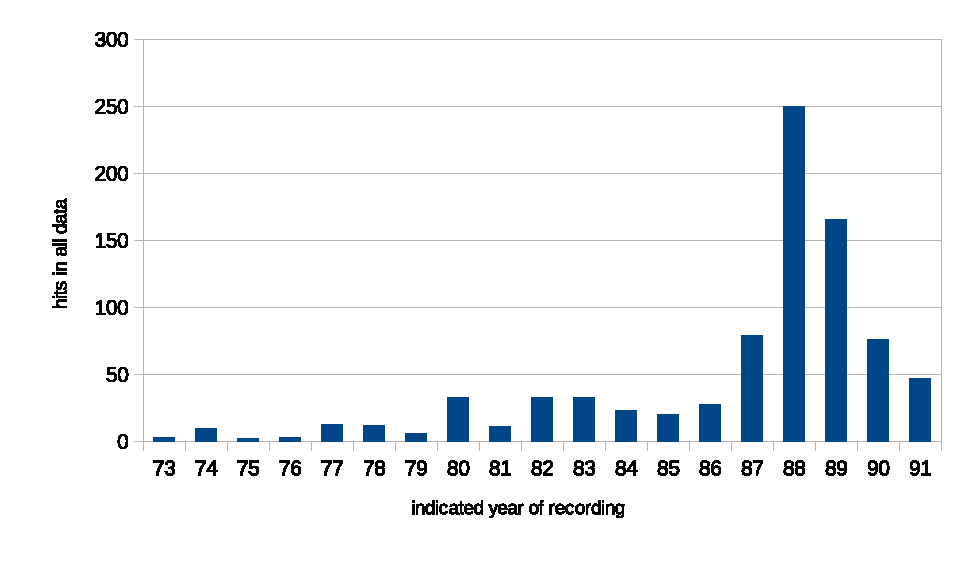
\includegraphics[scale=0.6]{rc/teresa-by-year.eps}
\caption{Number of hits for the query \texttt{terez.*} in the transcription by
alleged year of the recording}
\label{fig:teresa-year}
\end{figure}

The peak around the year 1988 supports the speculation that topics in the talks
correlate with those of books written at the same time.

\chapter{Acoustic Properties}
\label{chap:acoustics}

Automatic speech recognition is generally approached by means of machine
learning: a statistical model is inferred based on some training data. Its
application is based on the assumption that whatever was learned about the training
data will also apply to the input data. It is clear then, that if the input
data have different properties than the training data, the basic assumption is
violated and the inference performance will suffer.
Also, if the training data themselves are damaged in a way that makes the desired
information harder to extract, the learning is going to be less successful.

For speech recognition, the problem of noise, reverberation and other defects
has been a pain point and also a point of research. To mention some, Gillespie
and Atlas\cite{gillespie2002diversity} deal with reverberation for
GMM-based ASR, Yoshioka et al.\cite{reverbmagazine} summarize various
dereverberation techniques, Ko et al.\cite{reverbaugment} attempt to
simlulate reverberation in training data digitally. Seltzer, Yu and
Wang\cite{dnnnoiserobust} deal with noise in DNN-based ASR.

There are in principle two ways to deal with the negative effect of acoustic
deficiencies in speech recognition: 1) to adapt the model, which includes
training on augmented data, and 2) to adapt the input data. This chapter
presents experiments in the latter approach. See
section~\ref{sec:svolocz:svolocz} for an experiment with model adaptation.

\section{ASR Performance}

We are looking into the problem of acoustic inconsistencies in terms of varying
overall quality, reverberation, noise, overdrive and other phenomena in a
dataset that is to be automatically transcribed and listened to by humans.

Te heterogenous acoustic quality of the corpus affects both the speech recognition
performance and the listening experience. Let's look at speech recognition results
of a DNN-based model trained on manually transcribed parts of the corpus, as  described in chapter~\ref{chap:svolocz}. Whereas the word error rate on the
overall test set is 19\%, it is 45\% on a sample of recordings suffering from
overdrive, and 68\% on recordings taken on a magnetophone tape with a slow
recording speed of 2 centimeters per second after some 30 years of living-room
storage.

I am conducting an experiment to make the input data similar to the training
data instead of the more usual other way around because 1) it is not easy to
make the volunteer annotators transcribe acoustically flawed data, 2) not only
speech recognition would benefit from successful denoising, the listening
experience would improve too, and 3) the model could stay leaner.

What acoustic defects are actually present? Since the corpus was digitized from
magnetophone tapes of spontaneous talks of a single speaker recorded in various
amateur conditions and with consumer devices, we can broadly distinguish these
types of quality degradation:
\begin{enumerate}
\item{additive noise -- hum or hiss,}
\item{
    stationary interference like screeching added by low-quality magnetophone
    parts or the erasing head signal,
}
\item{non-stationary interference like background speech or door slams,}
\item{
    room echo or ill-equalized microphone boosting or cutting certain
    frequencies,
}
\item{non-linear distortion of the magnetophone}
\item{speed fluctuations.}
\end{enumerate}

The individual interference types affect each other and can occur several times
in several stages. For instance, the echo is essentially convolution with a certain vector of
amplitude values, known as the impulse response. It might even not be
constant if there are moving objects in the room or if the speaker or
microphone is moving. This convolution is followed by a non-linear
distortion in the microphone and its preamplifier and convolved again with
another impulse response, this time representing a frequency and phase
response of recorder's amplifiers. Finally it is non-linearly distorted in
the process of making a magnetic recording on the tape. Another batch of
distortions comes during the playback. On top of that, in every step a certain
amount of additive noise is introduced. Clearly, modeling, let alone reverting these
interferences is a difficult task.

\section{Denoising}

I conducted a baseline experiment employing the standard denoising based on
spectral subtraction. For each recording, a set of passages most likely
representing silence are extracted, a noise profile is calculated out of them,
and then subtracted from the spectrum.

Subjective evaluation confirms the expectable outcome that relatively
high-quality recordings that only suffer from some additive noise get
easier to listen to. Recordings suffering from other defects and overall lower
audio quality sometimes get rather harder to understand.

I have also trained a speech recognition system on the denoised data. The
performance has sunken to word error rate of 0.94, which basically means the
transcription doesn't work at all. Curiously enough, the
original model trained on non-denoised data performs much better on the denoised
test data with word error rate of 0.70. Table~\ref{tab:results-denoise} sums
these up.

\begin{table}[htpb]
\caption{Word error rate for the original and denoised test data by a model trained
on the original and denoised training data.}\label{tab:results-denoise}
\centering
\begin{tabular}{|l||r|r|}
\hline
WER    & original model & denoised model \\
\hline
original testing data & 0.189 & 0.940 \\
denoised testing data & 0.698 & 0.941 \\
\hline
\end{tabular}
\end{table}

\section{Neural Domain Transfer}

The revolutionary article of Zhu et al.\cite{cyclegan} presenting
cycle-consistent generative adversarial networks gave mankind a mighty tool and
a hilarious toy that was used for a variety of tasks reducible to
domain transfer.
Most closely related to the work presented in this article is probably
SEGAN\cite{pascual2017segan}: CycleGAN employed to enhance speech.

CycleGAN assumes two datasets in consistent domains: day and night photos,
schematic and photographic maps, male and female speech etc. In this case,
we have a clear consistent domain of clean, high-quality recordings and the
rest, which suffers from any combination of a number of defects. The damaged
recordings are very unlike each other, they don't form a consistent domain.

There are two ways of dealing with this situation: 1) adapt CycleGAN so that it
can deal with a ``compact'' and a ``scattered'' domain or 2) cluster the
data and apply CycleGAN on the individual clusters. While adapting CycleGAN may be a
point of future work, we have explored the simpler way of clustering the data.

\section{Clustering}

In order to perform clustering on any dataset, a metric on the data is needed.
I have used that proposed by Mandel \& Ellis\cite{mandel2005song}, which
is based on mel-frequency cepstra. A distance matrix has been created using
musly\cite{schnitzer2011using} and the clusters on top of that using
hierarchical clustering\cite{johnson1967hierarchical}.

A manual... or rather aureal check on the clusters confirms that files falling
into a cluster are indeed acoustically similar. So we arrived at a cluster of
overdriven recordings, a cluster of heavily hummed ones etc.

The experiment presented below is conducted on three clusters:
\begin{enumerate}
\item{A cluster of the cleanest recordings, used as the destination domain,}
\item{a cluster of overdriven recordings and}
\item{a cluster of recordings taken with low tape speed.}
\end{enumerate}
Recordings in cluster 3 are the hardest to understand even for humans. All these
clusters have a maximum internal distance of 25.

\section{Results}

I have used the voice transfer method as proposed by Kaneko \&
Kameoka\cite{kaneko2017parallel} and implemented by
Mao\footnote{github.com/leimao/Voice\_Converter\_CycleGAN}. I have trained
transfer 1) between the clean and the overdriven cluster and 2) between the
clean and the low-speed cluster.

After 200 epochs, I have performed speech recognition on the transferred data.
The result is summed up in Table~\ref{tab:results}.

\begin{table}[htpb]
\caption{Word error rate for the two damaged clusters before and after CycleGAN
transfer.}\label{tab:results}
\centering
\begin{tabular}{|l||r|r|}
\hline
           & original & transferred \\
\hline
overdriven & 0.450 & 0.441 \\
low-speed  & 0.685 & 0.939 \\
\hline
\end{tabular}
\end{table}

The word error rate decrease in the overdriven cluster is unfortunately statistically
insignificant with standard deviations 0.054 and 0.079 of the transferred and
original versions respectively. An important benefit is
that the transferred overdriven (or should we say de-overdriven) sound files are
much easier on the ear and it can be a help for human listeners.

The wrecking word error rate increase from 69\% to 94\% in case of the
recordings taken at low tape speed requires further investigation.
Figure~\ref{fig:plzen} shows the waveform and spectrum of a sample from the low-speed
cluster before and after the transfer. For comparison,
Figure~\ref{fig:overdrive} shows the same for the overdriven cluster.
Notice how parts of the signal are completely missing in the converted low-speed
sample. It seems that when the signal is too hard to separate from the noise,
the convertor prefers to generate silence.

I conclude that adapting the acoustically damaged data to be more likely to the
clean, in order to boost speech recognition performance, requires a much more
advanced engineering than conducted in these experiments. Enhancing the
listening experience seems significantly more reachable and can help us get
transcripts of the more problematic recordings. This would expand the training
data set to include examples of these problematic parts, probably decreasing the
word error rate. Confirming this remains a point of future work, though.

\begin{figure*}[tpb]
\centering
\includegraphics[width=0.9\hsize]{rc/plzen.eps}
\caption{Wave form (above) and spectrogram (below) of a recording taken in low
tape speed before the CycleGAN transfer (left) and afterwards (right).}
\label{fig:plzen}
\end{figure*}

\begin{figure*}[tpb]
\centering
\includegraphics[width=0.9\hsize]{rc/overdrive.eps}
\caption{Wave form (above) and spectrogram (below) of an overdriven recording
before the CycleGAN transfer (left) and afterwards (right).}
\label{fig:overdrive}
\end{figure*}

\chapter{Speech Recognition on Makoň's Corpus}
\label{chap:svolocz}

Acquiring a complete transcript of the given speech recordings is a central task
of this thesis. Furthermore, the method proposed assumes an initial transcript
to be present from the beginning. Therefore, developing a speech recognition
system for the data at hand was an ubiquitous task for me.

I have built the first system using HTK and have later switched over to
DeepSpeech, a system based on deep neural networks inspired by the 2014 Baidu
article\cite{hannun2014deep}.

In accordance with the architecture design, I have been using the ever-growing
set of manual transcripts for training the acoustic model. The seed transcript
has been taken by a model trained on some 15 minutes of material that I
transcribed myself.

Since there was not enough data to use as a gold standard for evaluation, I have
always separated some 10\% of then-available manual transcripts as a test set
(and another 10\% as development test set). For this reason, scores of the
individual models are not comparable. Only later during the development, I have
defined a standard evaluation set for testing purposes, which comprises of five
times ten minutes from various recordings across the corpus.

The best score reached by a HTK-based model on this set is 46.3\%, whereas the
best score reached by a DeepSpeech-based model is 19.2\%. These numbers
represent a kind of expectable performance level given the technology and data
used. There were many errors damaging the performance that had to be identified
and overcome. There were also many attempts to push the performance up above
this expected level, like tweaking the cepstral normalization, boosting or the
above-described acoustic pre-processing.

Finally, one obvious way of enhancing the performance led over widening the
training dataset. In chapter~\ref{chap:acoustics}, I stated there were two ways
to approach training and testing data inconsistency. There, I presented
experiments addressing adaptation of the training data. This experiment of
broadening the training data set realizes in fact the other branch.

\section{Extended Training Data}
\label{sec:svolocz:svolocz}

There are some free Czech corpora fit for speech recognition training, like
Vystadial\cite{vystadialarticle} with its 77 hours of VoIP calls
and Otázky Václava Moravce: 35 hours of transcribed recordings of the
Czech TV talk show\cite{ovmdata}.

There are also some that are not publicly, freely available but that can be used
anyway: Charles University
Corpus of Financial News (CUCFN, 65 hours)\cite{byrne1999large} and the Balanced
corpus of informal spoken Czech (Oral2013, 293 hours)\cite{oral2013} usable for
research purposes, and the spoken Bible (100 hours) available with no license
terms from \url{poslouchamebibli.cz}.

These provide some 500 hours of training data, which is five times as much as
available from the in-house transcripts. However, Oral2013 is a rather peculiar
set, as its acoustic quality and speech intelligibility are quite low. But there
is one more source of training data that remains to be untapped.

The Czech parliament meeting recordings represent a publicly available dataset
of high-quality audio recordings of contemporary Czech in consistent low-noise
audio quality worth almost 4000 hours of downloadable material, about 2800 hours
after subtraction of the overlaps. Extracting
training data for speech recognition systems would provide a corpus at least
one order greater in length than those so far publicly available.

Verily, I am not the first person to attempt using these recordings for speech
recognition. The Department of Cybernetics of University of West Bohemia
developed an automatic online subtitling system for the meetings in
2006\cite{pspsubs} and as a result, an 88-hour subset annotated by high-quality
automatic transcript has been released for speech recognition training
purposes\cite{pspdata}.

I attempt to use the official stenographic transcripts available for all the
talks so that it can be a new entry in the above list, on par in quality and
excelling in size.

\section{Data Preparation}

Since the source data is publicly available and in the public domain, I merely
provide the scripts for downloading and building the corpus. The algorithms and
parameters used are described in this section.

Regrettably, the data are to my best knowledge only available in human-readable
form. The transcript is not clearly distinguished in the markup and is
interlaced with metainformation. The scraper therefore uses heuristics based on
the markup and may omit parts of the transcript or include non-transcript.

\subsection{Alignment}

One of the obstacles in using the stenographic transcripts for training an ASR
system is the very loose alignment available. The recordings are all 14 minutes
long and have a 4-minute overlap. The corresponding transcript is thus aligned
in 10-minute blocks with a roughly 2-minute padding on each side of the audio.
Figure~\ref{fig:overlap} schematically shows the alignment of the stenographic
transcript to the audio and the overlap of the recordings.

\begin{figure*}[tpb]
\centering
\includegraphics[width=0.9\hsize]{rc/overlap.eps}
\caption{Alignment and overlap of audio files and transcript. The examples are
from Feb. 12th 2020 around 10 o'clock. The transcript corresponding to the
recording in the upper left covers audio positions 01:34 - 11:24. The one in the
lower right from 01:24 to 12:00.}
\label{fig:overlap}
\end{figure*}

Systems for aligning long audio segments to their transcripts already exist,
like that of Moreno et al.\cite{moreno1998recursive} or
Hazen\cite{hazen2006automatic}. They are both based on an already existing
automatically acquired transcript. I use this technique as well, though 
simplified and adapted to the task.

I have used the dataset mentioned above\cite{pspdata} to train a GMM-based ASR
system, using the stenographs as training data for a language model. Using these
models, a word-level-aligned transcript of the whole set of recordings has been
acquired.

The predicted transcript and the stenographic one have then been compared for
Levenshtein distance, determining the edit operations needed to transform one
into the other. For each predicted word, a reliability score is then
computed as 1 - unreliability where unreliability is the number of edit
operations taken on it divided by its length.
Figure~\ref{fig:align} shows how the stenographic transcript is aligned with the
audio on word level.

\begin{figure*}[htpb]
\includegraphics[width=0.9\hsize]{rc/align.eps}
\caption{Schema of aligning the audio to the stenographic transcript on word
level.}
\label{fig:align}
\end{figure*}

Nota bene, a GMM-based system was chosen for the initial transcript instead of
a DNN-based for three reasons: 1) Foremost, it is straightforward to obtain
precise alignment from a GMM-based system. 2) The training doesn't require so
much computational resources and data. 3) It isn't crucial to have maximum possible
accuracy in this stage.

\subsection{Training Samples Selection}

The aligned 14 minute long recordings are then split to segments fit for use as
training data for an acoustic model.
With the audio segmented and corresponding manual transcripts extracted, the
last step remaining is selecting which segments to include in the traning data.
Indeed, since the recordings have a 2-minute padding on each side for 10 middle
minutes, we must discard at the very least 29\%\footnote{Erroneously stated in
the thesis as 40\%, pointed out by the opponent.} of the segments. I use
criteria based on word reliability for including a segment in the data.

The solution readily yields a high-quality training dataset of 1144
hours. Of the total 539,057 segments, 142,530 (26\%) have been accepted to the
training dataset.

\section{ASR Based on the Dataset}

I have trained a standard DeepSpeech model with training :
development : test ratio of 18 : 1 : 1; batch size 50; learning rate 0.0001; dropout
rate 0.2. I trained a model for every individual source and finally one on the
concatenation.

The language model used was a pentagram model with pruned singleton trigrams,
tetragrams and pentagrams. The bulk of scraped transcriptions, including those
with no downloadable corresponding audio, was used as training data for the
language model.

Table~\ref{tab:csasr:results} shows the speech recognition
results for each corpus on test data from itself and on a common test set from
all the corpora.

\begin{table}[htpb]
\caption{Word error rate of speech recognition on the individual corpora and on
their concatenation.}
\centering
\begin{tabular}{|l||r|r|}
\hline
source    & WER on self & WER on all \\
\hline
bible     & 9.20\%  & 94.7\% \\
cucfn     & 31.6\%  & 72.8\% \\
makoň     & 30.4\%  & 77.3\% \\
oral2013  & 78.4\%  & 60.7\% \\
ovm       & 21.6\%  & 72.9\% \\
\textbf{parliament}
          & 7.89\%  & \textbf{36.0\%} \\
vystadial & 51.0\%  & 74.0\% \\
\hline
all       & 26.0\% & 26.0\% \\
\hline
\end{tabular}
\label{tab:csasr:results}
\end{table}

The 30\% word error rate for model trained on Makoň and tested on Makoň is reached when using the
generic language model. When using a language model trained solely on Makoň
data, the word error rate drops to 19\% reported above.

\subsection{Results on Makoň Corpus}

The final best performance on the Makoň test set was attained by training on the
concatenated set using heldout Makoň data for validation, followed by two
training iterations on the Makoň training set. This yielded the final best performace of 13.0\% word error rate.

The training dataset expansion has significantly brought down the word error
rate for acoustically defect parts. The reduction was from 45\% to 35\% on the
overdriven cluster and from 69\% to 42\% on the low-tape-speed cluster.

\chapter{Web Interface}

My aim is to have a transcription as good as possible for the purpose
of searching and further, higher-level processing of the data. There is a pool
of people interested in the talks, who on one hand are the force we can try to
employ and on the other hand are the consumers of our effort, our target group
so to speak.

The web application should therefore combine the two purposes: 1. serve its user
with making the content available in a manner as good as possible and 2. animate
the user to give as much and as high-quality contribution as possible.

To my best knowledge, there is no other project with a comparable setting.

\section{Description of the Web Application}

\subsection{Usage}

I have no special assumption of the user beyond basic computer usage skills and
understanding the audio. I assume no prior training. There is a manual for
clearing common points of confusion. The main message in it is that anything
that is to be transcribed, should be transcribed with respect to
phonetic precision, even if it results in nonsensical character strings.

Anything except words spoken by the one speaker of interest is to be left
untranscribed, including noise or speech by other persons\footnote{In the K.M.
corpus,
other speakers represent a negligible fraction but I may later add support for
speaker annotation.}. Incomprehensible words are to be left uncorrected
(the ASR output kept) if the phones are unclear. If the phones uttered are clear
but it is not clear what word was meant, the word may be transcribed
phonetically.

\subsection{Implementation}

The application consists of several views:
\begin{enumerate}
\item{the start page where all recordings are listed and each points to a detail
view,}
\item{the detail view, where a recording can be played back, its transcription
is displayed and can be corrected by the user,}
\item{the search page, where hits to a search query are listed and point to
corresponding positions in the recordings,}
\item{static pages with general information, contact etc.}
\end{enumerate}

I shall only discuss the detail view as the others are not relevant to this
paper. Figure~\ref{fig:scn1lab} shows the interface during playback.
The interface in the figures is conveniently shown in English, although in
reality it is in Czech.

\begin{figure}[htpb]
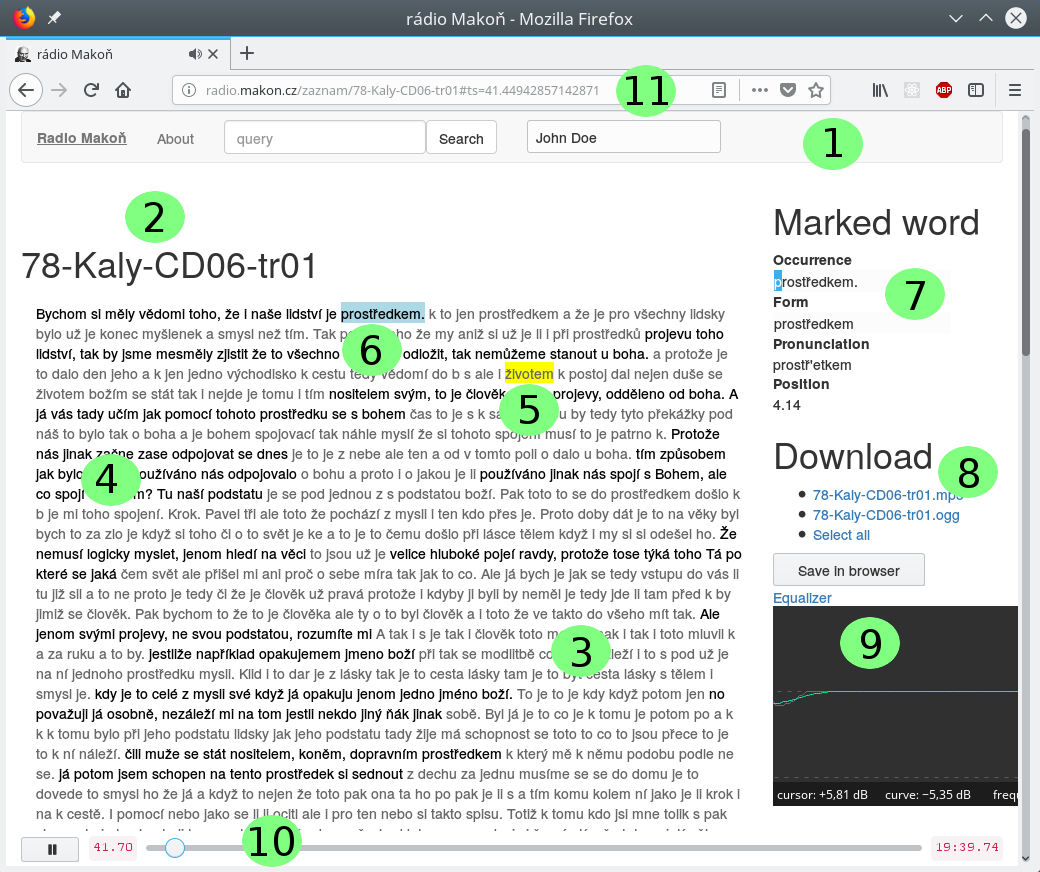
\includegraphics[scale=0.6]{rc/radio-makon-en-1-lab.png}
\caption{Web interface during playback}
\label{fig:scn1lab}
\end{figure}

Legend to Figure~\ref{fig:scn1lab}:
\begin{enumerate}
\item{
    Header with
    {app name linking to start page,}
    {about link,}
    {search field and}
    {username input field;}
}
\item{Identifier of the recording;}
\item{Automatically transcribed segments in grey;}
\item{Manually transcribed segments in black;}
\item{Currently played-back word highlighted by yellow background;}
\item{Marked word highlighted in regent st. blue;}
\item{Marked word info;}
\item{
    Tools for storing:
    {direct links to the audio files,}
    {selecting the whole transcription for easy pasting,}
    {storing the decoded recording in the browser's IndexedDB;}
}
\item{Graphical equalizer for compensating narrow-band noise;}
\item{Audio playback controls;}
\item{Current position reflected in URL fragment.}
\end{enumerate}

\subsection{Displaying the Transcription}

Many transcription programs show the transcription as a vertical list of
utterances, see Figure~\ref{fig:transcriber1} for an example of
Transcriber. I attribute this to the fact that the atomic elements of
the transcription are the user-entered utterances and their boundaries are
reliable. In our case, the atomic elements are words. There are sentences, sure,
but the segmentation to sentences by the ASR is very unreliable, so we want it
to be natural to transcribe a segment overlapping sentence boundaries.

\begin{figure}[htpb]
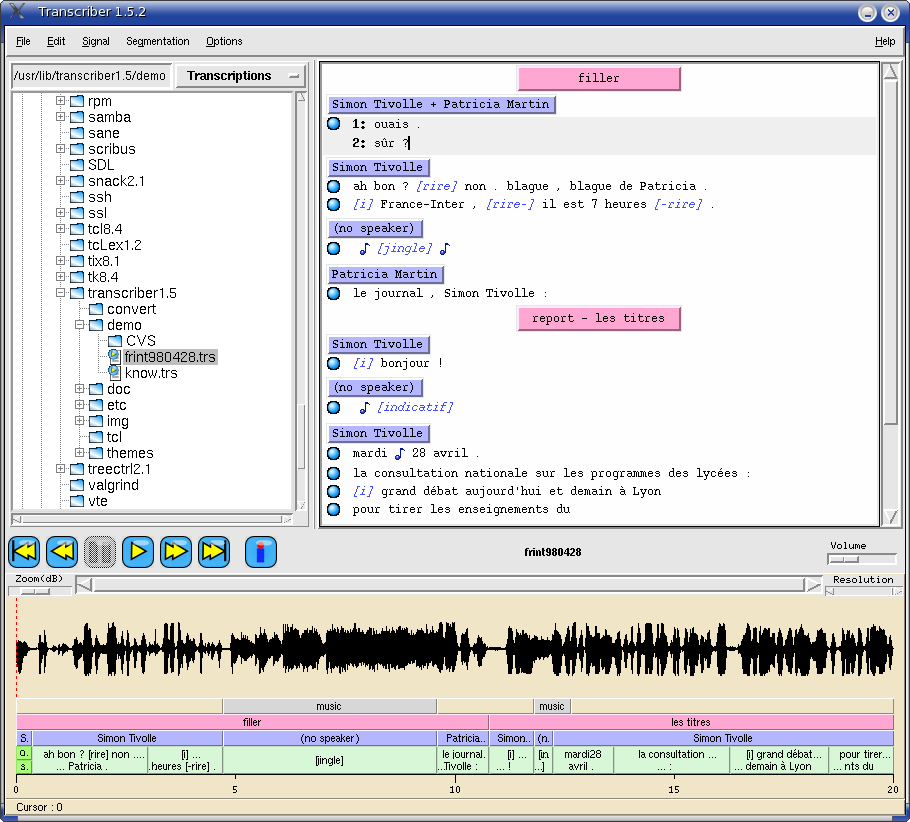
\includegraphics[scale=0.4]{rc/transcriber1.png}
\caption{A screenshot of Transcriber}
\label{fig:transcriber1}
\end{figure}

This is one of the reasons why we display the transcription basically as a
single wrapped line.

\chapter{Conclusion}

The main focus of this work has been developing a new method for enriching a
spoken corpus by a transcript layer. The method presented requires no paid
annotators and reckons with difficult material for which there is no solid
automated speech recognition available. As far as I know, all previous works
either employ paid annotators or use speech recognition as it is a-priori
available.

Not only a simple transcript is yielded but also another layer of phonetic
transcript, aligned with the source audio.

The method has been employed on the spoken corpus of Karel Makoň and proven
viable. The result is a complete coverage of the corpus with automatically
acquired transcript with an estimated word error rate of 13\%, which is on par
with the state of the art, considering the age, quality and spontaneity of the
recorded speech.

More importantly, the viability of the method has been proved by the fact that
108 hours of material have been successfully transcribed by lay, elderly users.

Not only has the method been developed, proven and described for benefit of
others who find themselves in a similar setting, but also software tools have
been created that can be freely re-used in a more or less similar setting.

As a
prominent point stands the web application allowing for work with a large set of
speech recordings, which enables browsing the material, listening with
synchronous display of the transcript, corrections of the transcript from the
user and several other advanced features, packed in a modern installation-free
web page.
It can be used in a variety of settings, wherever one of its distinct features
are required.

The toolchain for catalogizing the raw recordings into the web application,
turning the manual transcripts into training data, acquiring a speech
recognition system and running it on untranscribed data is split so
that data-dependent and data-independent parts are separated, allowing easy use
on new data. This has been done several times, on data described in this thesis,
like the Czech parliament meetings, as well as on data outside of this work.

Another software tool released in the course of this work is a tool for
turning the stenographed Czech parliament meetings into a training dataset for
speech recognition, bringing to the community a new corpus one order larger than other publicly
available datasets.

Other smaller but useful tools include expansion of numbers written as digits to
all possible Czech spellings, a library for parsing MFCC headers in Perl, a
script for denoising long sound files, including automatic extraction of
fitting silences, and others.

Finally, the available spoken corpus of Karel Makoň itself is an achievement of
this work. It is a unique resource that conserves the teachings of a Czech
spiritual capacity, that can now be studied and used as material by theologians,
historians, seekers, and also computational linguists and parties involved in
natual language and/or signal processing.

\bibliographystyle{unsrt}       %% [číslo]
\renewcommand{\bibname}{References}
\bibliography{citace}

%%% Seznam použité literatury

%%% Obrázky v disertační práci
%%% (pokud jich je malé množství, obvykle není třeba seznam uvádět)

%%% Tabulky v disertační práci (opět nemusí být nutné uvádět)
%%% U matematických prací může být lepší přemístit seznam tabulek na začátek práce.

%%% Použité zkratky v disertační práci (opět nemusí být nutné uvádět)
%%% U matematických prací může být lepší přemístit seznam zkratek na začátek práce.
%\chapwithtoc{Seznam použitých zkratek}

%%% Součástí doktorských prací musí být seznam vlastních publikací
\chapter*{List of Publications}
\addcontentsline{toc}{chapter}{List of Publications}

\begin{enumerate}
\item{
    Oldřich Krůza and Nino Peterek.
    Making Community and ASR Join Forces in Web Environment.
    In \textit{International Conference on Text, Speech and Dialogue},
    pages 415--421.
    Springer, 2012.
}
\item{
    Oldřich Krůza and Vladislav Kuboň.
    Second-Generation Web Interface to Correcting ASR Output.
    In Kohei Arai, Rahul Bhatia and Supriya Kapoor, editors,
    \textit{Proceedings of the Future Technologies Conference (FTC) 2018},
    number 1, pages 749--762, Cham, Switzerland, 2018.
    Science and Information Organization, Springer-Verlag.
}
\item{
    Oldřich Krůza.
    Phonetic Transcription by Untrained Annotators.
    In Stanislav Krajči, editor,
    \textit{Proceedings of the 18th conference ITAT 2018:
    Slovenskočeský NLP workshop (SloNLP 2018)},
    volume 2203 of \textit{CEUR Workshop Proceedings},
    pages 35--40,
    Košice, Slovakia, 2018.
    Šafárik University, Košice,
    CreateSpace Indepedent Publishing Platform.
}
\item{
   Jan Oldřich Krůza.
   Spoken Corpus of Karel Makoň.  
   In \textit{Book of Abstracts XI International Conference on Corpus Linguistics},
   pages 189--190.
   ADEIT - Fundación Universidad-Empresa de la Universitat de València, 2019.\\
   \texttt{https://adeit-estaticos.econgres.es/19\_CILC/book\_abstracts.pdf}
}
\item{
  Jan Oldřich Krůza.
  Czech parliament meeting recordings as ASR training data.
  In \textit{Proceedings of the 2020 Federated Conference on Computer Science
  and Information Systems (FedCSIS)}.
  Pending.
}
%\item{
%    Jan Oldřich Krůza.
%    Restructuring Spoken Corpus for Streaming Emulation.
%    In \textit
%}
\end{enumerate}

%%% Přílohy k disertační práci, existují-li. Každá příloha musí být alespoň jednou
%%% odkazována z vlastního textu práce. Přílohy se číslují.
%%%
%%% Do tištěné verze se spíše hodí přílohy, které lze číst a prohlížet (dodatečné
%%% tabulky a grafy, různé textové doplňky, ukázky výstupů z počítačových programů,
%%% apod.). Do elektronické verze se hodí přílohy, které budou spíše používány
%%% v elektronické podobě než čteny (zdrojové kódy programů, datové soubory,
%%% interaktivní grafy apod.). Elektronické přílohy se nahrávají do SISu a lze
%%% je také do práce vložit na CD/DVD. Povolené formáty souborů specifikuje
%%% opatření rektora č. 72/2017.
%\appendix
%\chapter{Přílohy}

%\section{První příloha}

\openright
\end{document}
